\documentclass{article}
\usepackage{listings}
\usepackage{mathrsfs}
\usepackage[utf8]{inputenc}
\usepackage{amssymb}
\usepackage{lipsum}
\usepackage{amsmath}
\usepackage{fancyhdr}
\usepackage{geometry}
\usepackage{scrextend}
\usepackage[english,german]{babel}
\usepackage{titling}
\setlength{\droptitle}{-3cm}
\usepackage{tikz}
\usepackage{algorithm,algpseudocode}
\usepackage[doublespacing]{setspace}
\usetikzlibrary{datavisualization}
\usetikzlibrary{datavisualization.formats.functions}
\usepackage{polynom}
\usepackage{amsmath}
\usepackage{gauss}
\usepackage{tkz-euclide}
\usetikzlibrary{datavisualization}
\usetikzlibrary{datavisualization.formats.functions}
\author{
Alexander Mattick Kennung: qi69dube\\
Kapitel 1
}
\usepackage{import}
\date{\today}
\geometry{a4paper, margin=2cm}
\usepackage{stackengine}
\parskip 1em
\newcommand\stackequal[2]{%
  \mathrel{\stackunder[2pt]{\stackon[4pt]{=}{$\scriptscriptstyle#1$}}{%
  $\scriptscriptstyle#2$}}
 }
\makeatletter
\renewcommand*\env@matrix[1][*\c@MaxMatrixCols c]{%
  \hskip -\arraycolsep
  \let\@ifnextchar\new@ifnextchar
  \array{#1}}
\makeatother
\lstset{
  language=haskell,
}
\lstnewenvironment{code}{\lstset{language=Haskell,basicstyle=\small}}{}
\usepackage{enumitem}
\setlist{nosep}
\usepackage{titlesec}
\usepackage{ stmaryrd }
\usepackage{verbatim}


\titlespacing*{\subsection}{0pt}{2pt}{3pt}
\titlespacing*{\section}{0pt}{0pt}{5pt}
\titlespacing*{\subsubsection}{0pt}{1pt}{2pt}
\title{Vorlesung 4}


\begin{document}
	\maketitle
	\[f^Y(y)=\frac{1}{2\pi\sigma_1\sigma_2}e^{-\frac{(y_1-\mu_1)}{2\sigma_1^2}-\frac{(y_2-\mu_2)}{2\sigma_2^2}}\]
	ist eine 2d Normalverteilung.\\
	\underline{gemeinsame} Dichte ist gegeben\\
	s.t.u $Y_1,Y_2$\\
	ja, in zwei unabhängige Dichten aufteilen(multiplikation geht)\\
	Randdichten\\
	\[f^{Y_1}(y)=\int_\mathbb{R}\frac{1}{2\pi\sigma_1\sigma_2}e^{-\frac{(y_1-\mu_1)}{2\sigma_1^2}-\frac{(y_2-\mu_2)}{2\sigma_2^2}} dy_2 = \frac{1}{\sqrt{2\pi}\sigma_1}e^-\frac{(y_1-\mu_1)}{2\sigma_1^2}\int_\mathbb{R}\frac{1}{\sqrt{2\pi}\sigma_2}e^{-\frac{(y_2-\mu_2)}{2\sigma_2^2}} dy_2 = \frac{1}{\sqrt{2\pi}\sigma_1}e^-\frac{(y_1-\mu_1)}{2\sigma_1^2}\]
	weil links eine Normalverteilung über $\mathbb{R}$ integriert wird.\\
	Stochastisch unabhängige $Y_1\dots Y_n$ impliziert:\\
	kommutativität der Zufallsvariablen.\\
	Teilmengen sind stochastisch unabhängig.\\
	disjunkte Gruppen sind stochastisch unabhängig $(Y_1,Y_3)$ und $(Y_4,Y_5)$\\
	messbear Funktionen von stoch.unabhängigen ZV z.B. $g(Z_1)=Y_1+2Y_3^2$ und $h(Z_2)=Y_4\cdot e^{Y_5}$\\
	jede konstante ZV ist von anderen ZV stoch.unabhängig.\\
	sind $Y_1\dots Y_{n-1}$ unabhängig und sind $(Y_1\dots Y_{n-1}), Y_n$ stoch. unabh., dann auch $Y_1\dots Y_n$ stochastisch unabhängig.\\
	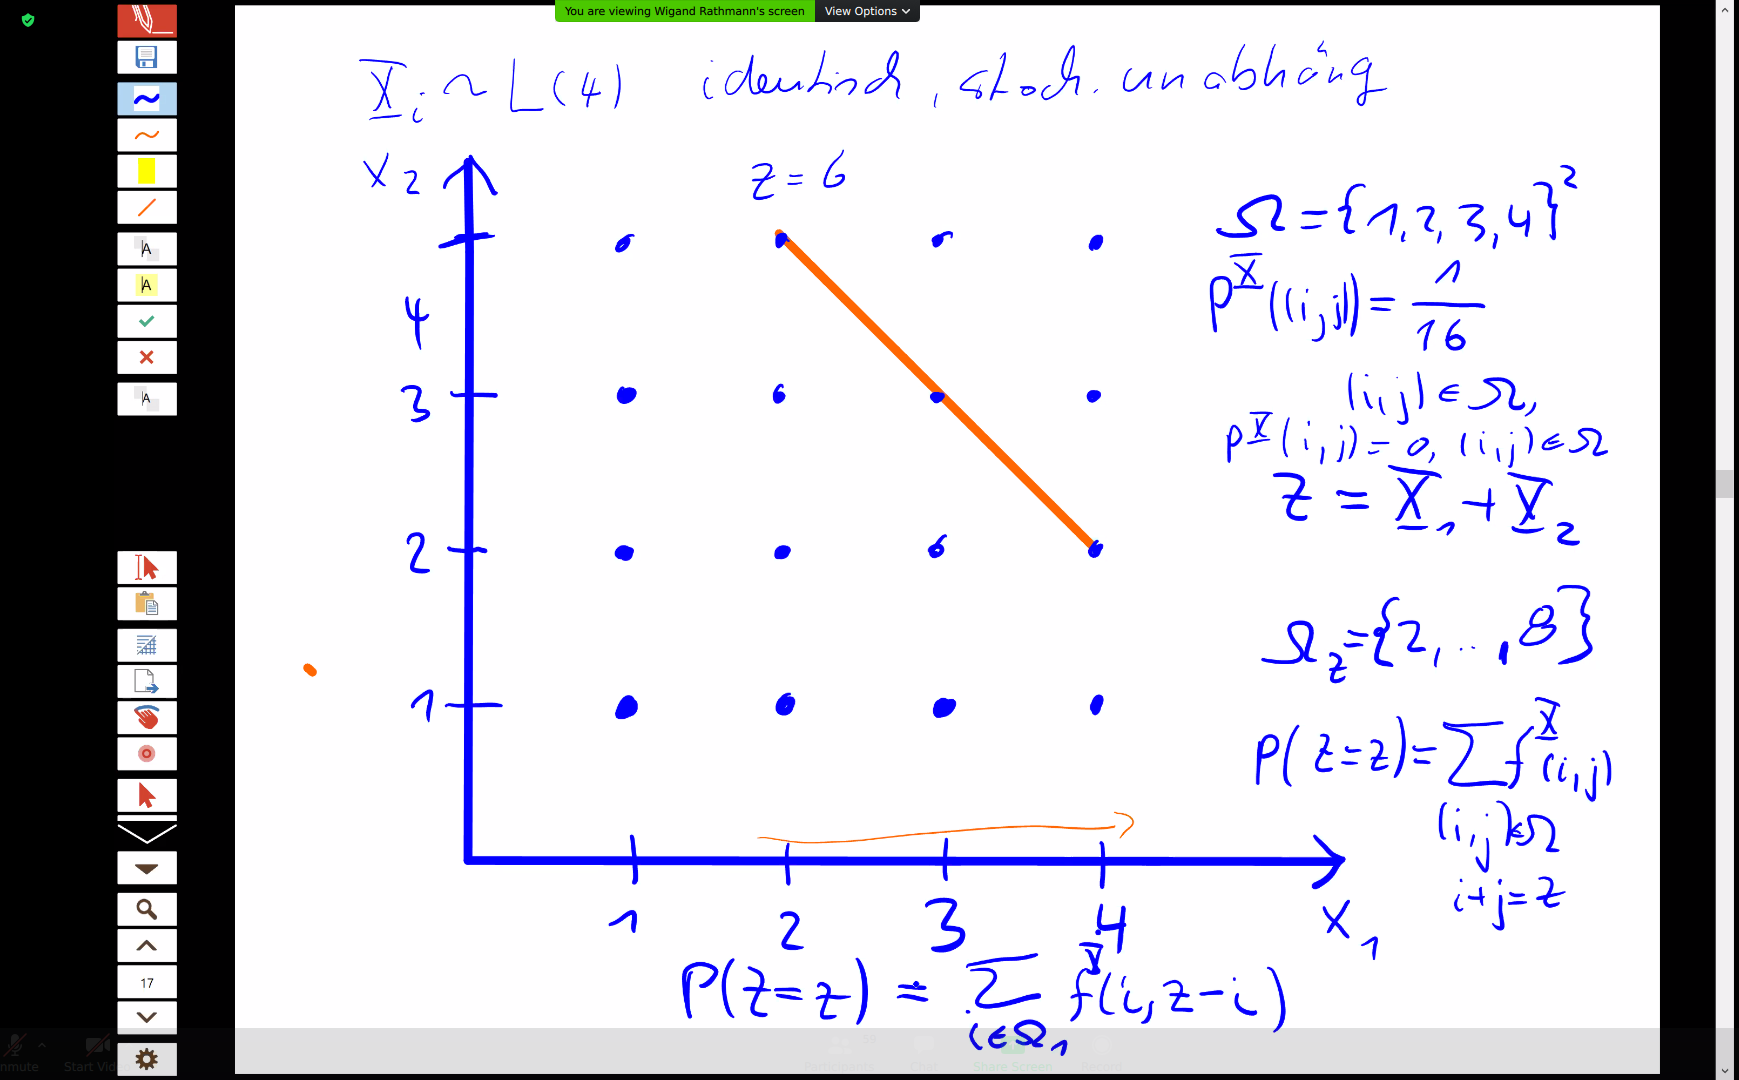
\includegraphics[width=256px]{laplaceIID.png}\\
	sprich, weil z=i+j, können wir, wenn wir z wählen für jedes i ein zugehöriges j finden.
	dieses muss $j=z-1$\\
	\[P(Z=z) =\sum_{i\in\Omega_1} f(i,z-i)\]
	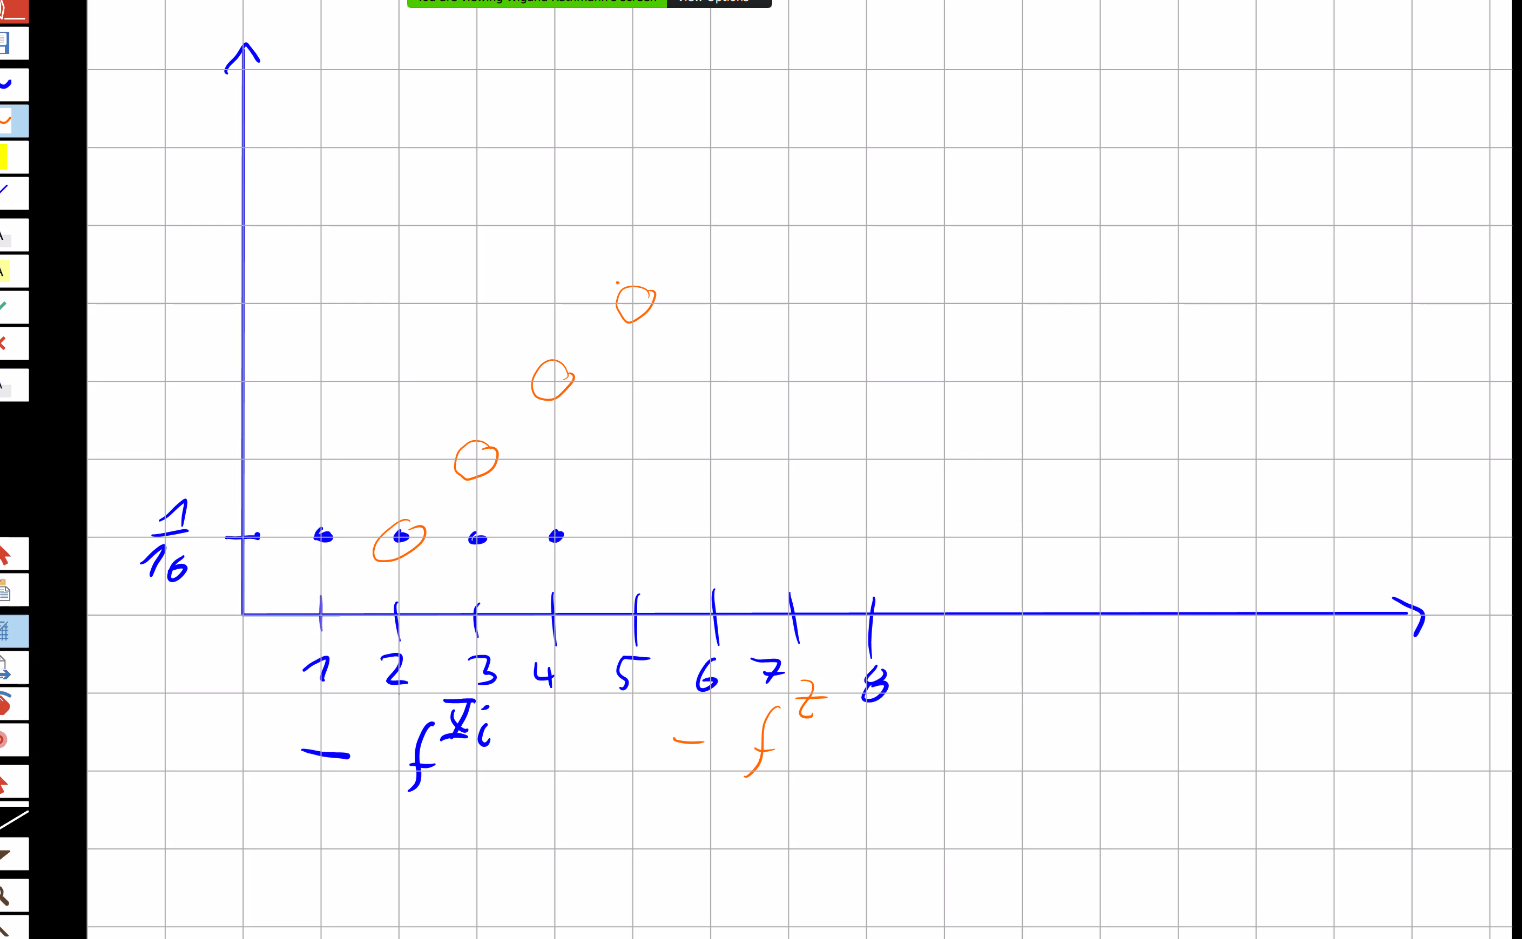
\includegraphics[height=256px]{z-Prob-Graph.png}\\
	man kann hier schon den Zentralen Grenzwertsatz sehen: Wenn wir unendlich viele iid variablen addiert hätten, hätten wir hier eine Normalverteilung.\\
	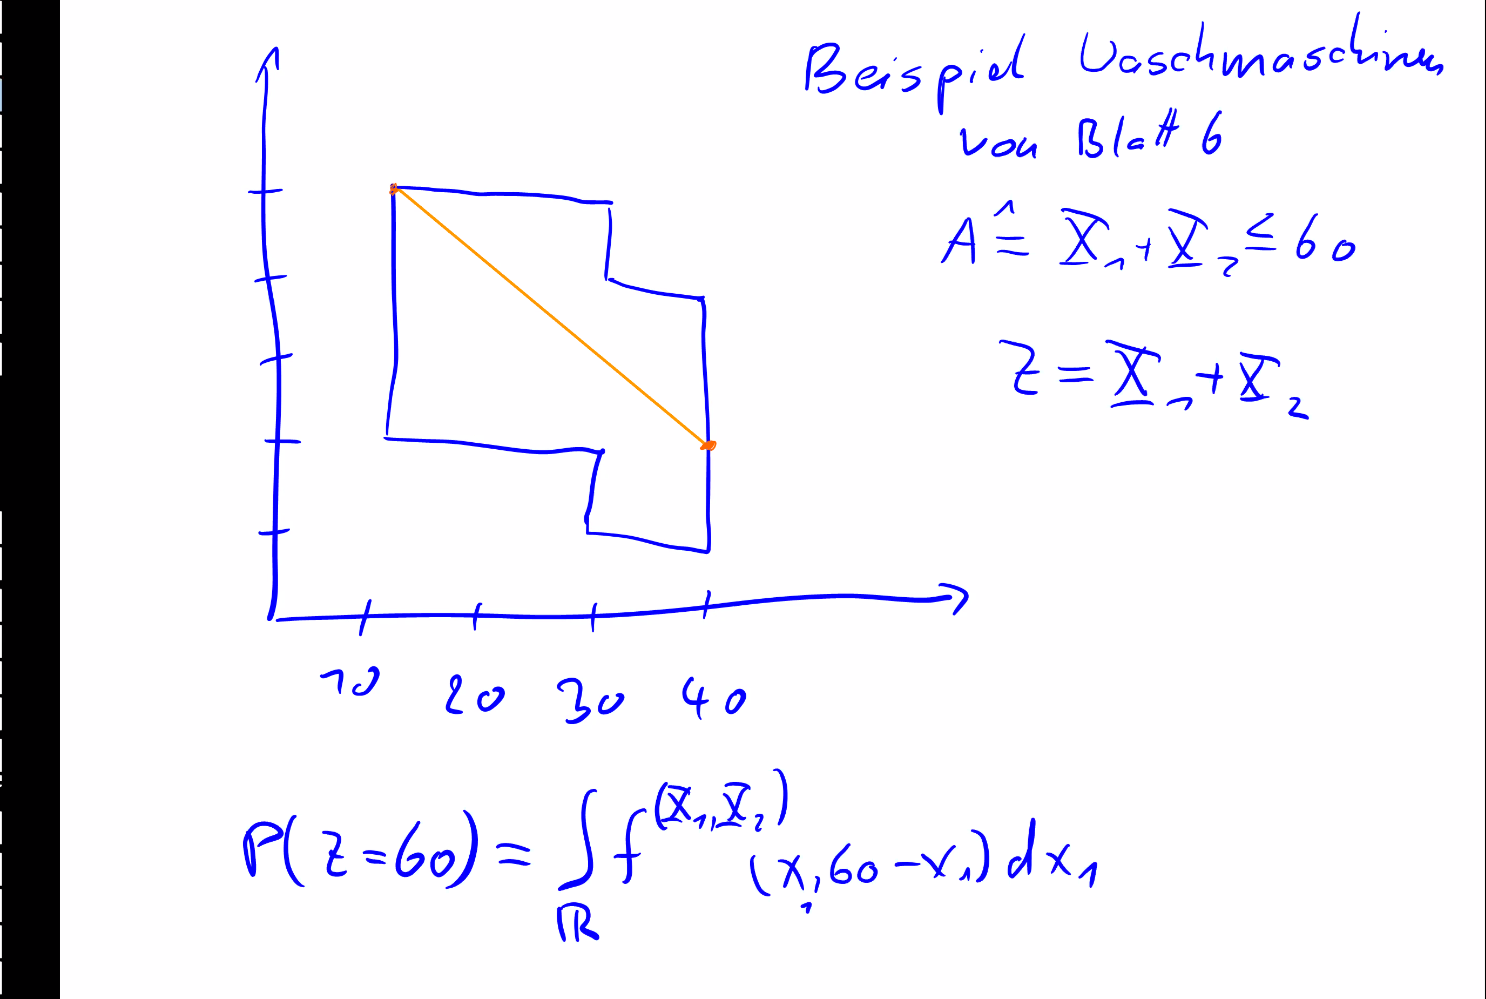
\includegraphics[width=256px]{kontinuierlicheFaltung.png}\\
	\[P(Z=z)=\int_\mathbb{R} f^X(x)f^Y(z-x)\]
	WICHTIG: beide können verschieden Verteilt sein, müssen aber stochastisch unabhängig sein.\\
	Beispiele:\\
	N-fach wiederholte Bernoulli-Experimente liefern die Binomialverteilung:\\
	\[B(n,p)=B(p)*\dots B(p)\]
	Die Poisson-Verteilung ist über faltung abgeschlossen:
	\[\pi(\lambda_1)*\pi(\lambda_2)=\pi(\lambda_1+\lambda_2)\]
	Die Geometrische verteilung liefert durch faltung die negative binomialverteilung (wahrscheinlichkeit k-hits zu erhalten ist summe einen hit zu erhalten k-mal)
	\[Nb^+(k,p)=\underbrace{Geo^+(p)*\dots*Geo^+(p)}_{k\ mal}\]
	Die Faltung zweier beliebiger Normalverteilter ZV ist wieder Normalverteilt (abschluss unter faltung)
	\[\mathcal{N}(a,\sigma^2)+\mathcal{N}(b,\tau^2) = \mathcal{N}(a+b,\sigma^2+\tau^2)\]
	Bei Faltung von zwei Gamma-Verteilungen mit gleichem Parameter $\alpha$ ergibt
	\[\Gamma_{\alpha,\mu}*\Gamma_{\alpha,\tau}=\Gamma_{\alpha,\mu+\tau}\]
	Daraus folgen sonderfälle
	\[Exp(\alpha)=\Gamma_{\alpha,1}\]
	\[\Chi_1^2=\Gamma_{0.5,0.5}\]
	Daraus folgt
	\[Exp_n(\alpha)=\underbrace{\Gamma_{\alpha,1}*\dots* \Gamma_{\alpha,1}}_n\]
	\[\Chi_1^n=\underbrace{\Gamma_{0.5,0.5}*\dots *\Gamma_{0.5,0.5}}_n\]

\end{document}